\section{Prototype}
\textbf{Arkitekturen av det foreslåtte systemets logiske deler er beskrevet tydelig. \\
Valgt teknologi og rammeverk er beskrevet tilstrekkelig.}
\subsection{Beskrivelse av systemet}
Prototypen inneholder det vi har sett på som den viktigste funksjonaliteten. For å få mest mulig verdi ut av prototypen har vi med det begrenset den til å blant annet ikke inneholde en komplett løsning av betalingssystemet. Sikkerheten er også begrenset da prototypen kun skal være en mal på hvordan systemet kan bli utviklet videre.

\begin{figure}[H]
    \centering
    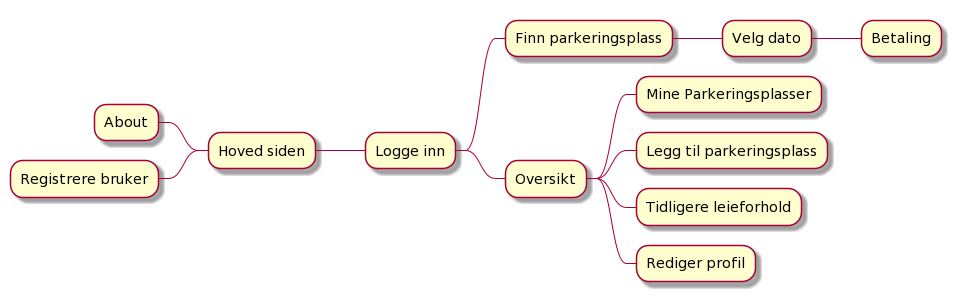
\includegraphics[width=12cm]{bilder/uml/oversikt.png}
    \caption{Oversikt over sidene i systemet}
    \label{fig:proto_overview}
\end{figure}
Figur \ref{fig:proto_overview} viser hvordan det er mulig å navigere rundt i systemet. Det meste av funksjonaliteten er lukket bak "Logge inn" siden for å begrense hva en hvilken som helst person kan se og hente ut av systemet. "About" og "Hovedsiden" inneholder ingen sensitiv informasjon og er tilgjengelig for alle for å gi en beskrivelse av hva systemet er. Deretter kan en bruker eventuelt velge å opprette en profil og få tilgang til systemet.

\subsubsection{Funksjonalitet og avgrensinger} 
\textbf{Tydelig hva slags krav som er dekket av prototypen }
Vi ønsker at prototypen skal vise det vi anser som den mest sentrale delen. Vi ønsker at den skal vise et MVP (Minimal viable product) hvor kunden kan få mest utbytte av prototypen tidligst mulig. Vi har sett på de ulike funksjonalitetene vi vil ha med, og kommet fram til ulike krav som er viktige i prototypen. Vår estimering utgjort i tabell \ref{tab:Kravestimering} har hjulpet oss med å se hva som bør prioriteres i prototypen og hva som kan tas med til senere utvikling. Våre User cases i seksjon \ref{user_case} har også bidratt til å avdekke den viktigste funksjonaliteten i systemet. Muligheten til å leie og legge ut en parkeringsplass er sentrale funksjoner som gir kunden mest utbytte og mulighet til å bruke prototypen, og dermed viktig å ha med i prototypen. Muligheten til å søke etter parkeringsplasser er også inkludert sammen med andre krav som gjør brukervennligheten av tjenesten bedre, slik at kunden kan få enda mer ut av prototypen. For vår prototype har vi valgt å fokusere på disse kravene:   

%Vi ønsker at prototypen skal vise det vi anser som den mest sentrale delen. Vi ønsker at den skal vise MBP hvor da kunden kan få mest utbytte av prototypen. Dermed har vi sett på de ulike funksjonalitetene vi vil ha med, og kommet til ulike krav som er viktige i prototypen. Som det å leie og legge ut en parkeringsplass er veldig viktige funksjoner som gir kunden mer utbytte og mulighet til å bruke prototypen. Vi har også valgt å inkludere krav som gjør brukervennligheten til kunden bedre, blant annet søk på parkeringsplasser.
For vår prototype har vi valgt å fokusere på disse kravene:
\begin{table}[H]
% \centering
\begin{tabular}{ll}
4.1.1.a & Opprette bruker m/ epost-adresse        \\
4.1.2.a & Logge inn m/ epost-adresse              \\
4.1.2.d & Feilmelding ved feil brukernavn/passord \\
4.1.3  & Legge inn parkeringsplass               \\
4.1.5  & Leie parkeringsplass                    \\
4.1.6  & Søk av parkeringsplass                  \\
4.1.7  & Brukerprofil                            \\
4.1.9  & Betaling                               
\end{tabular}
\end{table}
% \begin{itemize}
%     \item 4.1.1.a Opprette bruker m/ epost-adresse
%     \item 4.1.2.a Logge inn m/ epost-adresse
%     \item 4.1.2.d Feilmelding ved feil brukernavn/passord
%     \item 4.1.3 Legge inn parkeringsplass
%     \item 4.1.5 Leie parkeringsplass
%     \item 4.1.6 Søk av parkeringsplass
%     \item 4.1.7 Brukerprofil
%     \item 4.1.9 Betaling
% \end{itemize}
%\textit{* $\longrightarrow$ Her har vi fokusert på generelt for utleiere og ikke firma.} \\
%\textit{** $\longrightarrow$ Vi har valgt en lettere implementasjon, istedenfor kart er det poststed}\\
%\textit{*** $\longrightarrow$ Vi har valgt å vise oversikt over leide plasser og utleide plasser. Admin oversikt er ikke implementert, heller ikke oversikten vist med grafer.}\\
%\textit{**** $\longrightarrow$ Hoved kravet blir implementert, men ikke underkravene}
\vspace{-1em}
For hvert av disse kravene vil de mest viktigste delene bli implementert. Ergo de kravene som tidligst gir produkt til kunden. Det medfører at noen krav ikke blir implementert, blant annet administrator sine rolle i tjenesten og oversikten over inntjeninger i form av kakegraf.. 

 Brukere kan heller ikke se antall utilgjengelig og tilgjengelig plasser. Vi har implementert det slik at for en gitt adresse er det bare en parkeringsplass. Det medfører at Firma sin rolle ikke er implementert.


For krav om betaling er det hovedkravet som er i fokus. Det er da en demo av betalingsløsningen. Det medfører at betalingen er implementert med en enkel funksjon i vårt system som bestemmer om betalingen blir godkjent eller ikke. Dette kan bli implementert senere med de eksterne avhengighet som vi har valgt.
Det er også i fokus brukeren betaler for parkeringsplassen. Det medfører at firma ikke betaler for tjenesten eller at man ikke kan avbestille parkeringsplassen. Det kan bli implementert senere, og er ikke i fokus i vår prototype. Avbestilling også blir ikke prioritert, eller tjenesten sin konto. 


Søk av parkeringsplass er implementert i form av poststed. 


%Disse avgrensningene er listet under::
%\begin{enumerate}

%\item Systemet har kun en demo av en betalingsløsning. Det medfører at betalingen er implementert med en enkel løsning. Det er en enkel funksjon implementert i vårt system som bestemmer om betalingen blir godkjent eller ikke.

%\item Det er ikke implementert en avgiftsløsning for firmaer (prosentandel av salget) 

%\item Admin sin rollen er ikke implementert.

%\item Firma funksjonene er ikke implementert.
%\item Bruker kan ikke avbestille parkeringstjenesten.
%\item Søk av parkeringsplass har bare blitt implementert i form av poststed og ikke kart
%\end{enumerate}


\subsubsection{Modellering av prototypen}
\textbf{Diagrammer som beskriver relevatne deler av systemet eller prosessene (ikke nødvendigvis funksjoner i prototype). Elementene i diagrammene og funksjonaliteten deres er tydelig.}

Denne seksjonen vil vise modelleringen av prototypen og systemet. Det viser hvordan systemet/prototypens funksjoner samhandler. Det gjøres med forskjellige diagrammer som flytdiagram, aktivitetsdiagram, sekvensdiagram og lignende.
\paragraph{Opprette bruker modellering}
\begin{figure}[H]
    \centering
    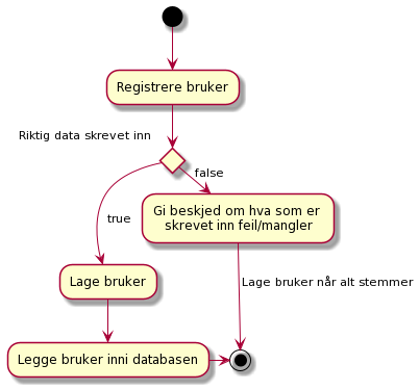
\includegraphics[width=5cm]{bilder/uml/registerebruke.png}
    \caption{Sekvensdiagram for opprette bruker}
    \label{fig:reg_bruker}
\end{figure}
Figur \ref{fig:reg_bruker} viser flyten i hvordan man registrerer en bruker. Dette kommer fra kravet 4.1.1.a hvor brukeren kan opprette en bruker med epost-adressen. Brukeren sender inn dataen sin via et skjema, systemet sjekker opp om dataen er skrevet inn riktig (om noe mangler, om det er riktig e-post og riktig telefonnummer), og hvis alt stemmer så blir profilen dannet og sendt videre til databasen. Hvis noe av informasjonen ikke er riktig så får brukeren beskjed om det slik at han kan rette det opp. 

Brukeren som blir registrert blir lagret i en json-fil istedenfor en database i vår prototype. Vi har gått for en litt mer lettvint løsning når det gjelder lagring av dataen, men siden fungerer fullstendig bortsett fra det.  

 
\paragraph{Logge inn modellering}

\begin{figure}[H]
\centering
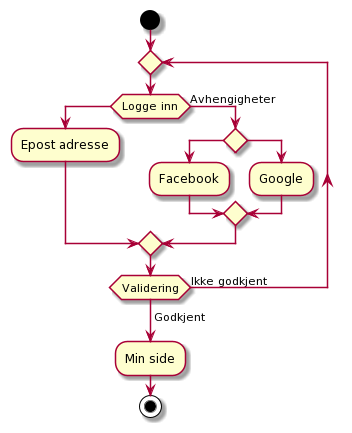
\includegraphics[width=5cm]{bilder/uml/loggeinn.png}
\caption{Aktivitetsdiagram for funksjonen å logge inn}
\label{fig:logginn}
\end{figure}
Figur \ref{fig:logginn} viser hvordan flyten skal være ved å logge inn. Dette kommer fra kravet 4.1.2 hvor da brukeren kan logge seg inn med enten Facebook, Google eller med epost-adresse. Figuren viser visuelt hvordan brukeren ser aktiviteten i kravet. Ved å logge inn blir det validert. Hvis det ikke blir godkjent blir man sendt til logge inn siden igjen. Hvis man får godkjent kommer man til Min side.

Facebook og Google er en ekstern avhengighet som vil da direkte komme til siden til facebook eller Google for å logge inn. I vår prototype er ikke dette implementert, da epost adresse innlogging gir verdi tidligst mulig for kunden. Dette er beskrevet i seksjonen om vår funksjonalitet og avgrensning av systemet.

\paragraph{Brukerprofil}
\begin{figure}[H]
    \centering
    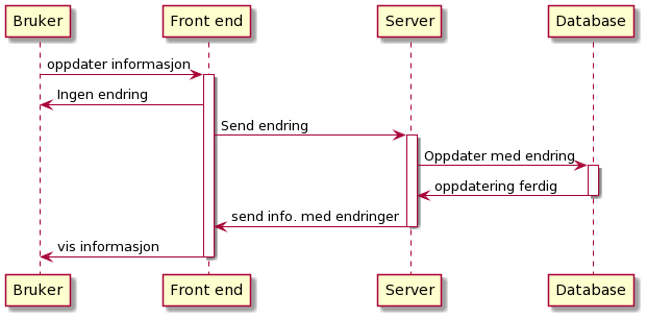
\includegraphics[width=10cm]{bilder/uml/brukerprofil.png}
    \caption{Sekvensdiagram for funksjonen endre informasjonen om brukeren lagret i vårt system }
    \label{fig:endre_bruker}
\end{figure}
Figur \ref{fig:endre_bruker} viser hvordan man gjør endring i brukerprofil. Skulle en bruker trykke på oppdater uten å ha gjort noen endringer kuttes prosessen av for å ikke gi unødvendig mye jobb for serveren. Videre sendes endringene til serverene som oppdaterer informasjonen i databasen. Når dette er gjort sendes den oppdaterte informasjonen tilbake til brukeren og vises i front end.

\paragraph{Søking av parkeringsplass}
\begin{figure}[H]
    \centering
    \includegraphics[width=5cm]{bilder/uml/søkeparkering.png}
    \caption{Aktivitetsdiagram for søking av parkeringsplass}
    \label{fig:search_parking}
\end{figure}
Figur \ref{fig:search_parking} viser hvordan brukeren oppfatter søking av parkeringplass fra krav 4.1.6 som omhandler å søke etter parkeringsplass. Det gir et visuelt bilde for brukeren hvordan søkingen går. De henter parkeringsplassene utifra poststedet eller lokasjonen i kartet. Disse hentes fra databasen.

I figuren ser du tydelig at man kan søke ved hjelp av kart. Dette gjør det lettere å finne nærmeste lokasjon. Det er også et ønske å sortere de etter visse egenskaper som for eksempel pris.

Vår prototype har fokusert på selve søkingen i form av poststed. 
\paragraph{Legge ut parkeringsplass}
\begin{figure}[H]
    \centering
    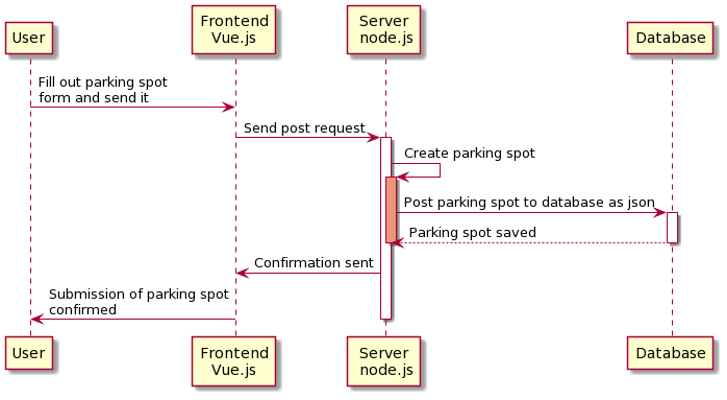
\includegraphics[width=10cm]{bilder/uml/legge_parkeringsplasss.png}
    \caption{Sekvensdiagram for legge ut parkeringsplass}
    \label{fig:legge}
\end{figure}
Figur \ref{fig:legge} viser til krav 4.1.4 som omhandler det å legge ut en parkeringsplass. Figuren viser at brukeren sender inn et skjema med data på nettsiden. Vue.js sender det videre til backend-en og oppretter en parkeringsplass. Parkeringsplassen blir sendt som json-data til databasen, og systemet sender en bekreftelse tilbake om at parkeringsplassen er lagt inn. På denne måten kan brukeren være sikker at alt ble gjennomført og parkeringsplassen er lagt inn siden det kommer en bekreftelse tilbake til brukeren som vist på figuren. 

Dette kravet er implementert fullstendig i vår prototype og fungerer som det skal. Vi har valgt å lagre dataen i en json-fil istedenfor en database for å gjøre løsninga mer lettvint.  
 
\paragraph{Betaling}
\begin{figure}[H]
    \centering
    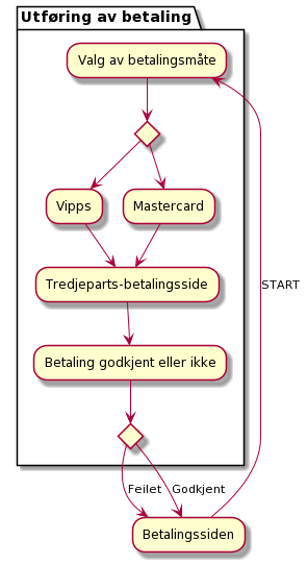
\includegraphics{bilder/uml/betaling.png}
    \caption{Flytdiagram for betalingen}
    \label{fig:betaling}
\end{figure}

En viktig del av systemet vil være betaling for tjenestene. Figur \ref{fig:betaling} viser hvordan betalingsdelen av systemet vil fungere. Dette kommer fra krav 4.1.8. Prototypen er en enkel versjon av systemet hvor betalingensdelen er avgrenset. En full versjon av betalingen vil kreve avtaler med Vipps og Mastercard.  

Først verifiseres det at «produktet» som skal bli kjøpt er tilgjengelig og at betalingsinformasjonen stemmer. Deretter velger kunden betalingsmåte og blir ført videre til den spesifikke betalingssiden. I prototypen blir det steget hoppet over og det vil bli gitt en direkte beskjed om godkjent eller feilet betaling. 




\subsubsection{Avhengigheter}
Noen av avhengighetene vi har er: 
\begin{enumerate}
    \item Javascript ES9 

    \item Vue.js 2.x

    \item BULMA som er et CSS rammeverk 

    \item Express rammeverk for å håndtere forespørsler 

    \item Versjon 14.13.0 av Node.js 

    \item  Jest rammeverk til testing 

    \item Pakkesystem npm som er en del av Node.js 
\end{enumerate}




\subsubsection{Kjente svakheter og problemer}
% \textit{Forklar ev. kjente svakheter og problemer med prototypen. Det er bedre at Kunden vet
% om problemer på forhånd før de ev. merker dem selv.}
% I og med at vårt produkt er en prototype, så er ikke alle kravene implementert, og heller er ikke systemet feilfritt. I vår prototype er det noen svakheter som
% \begin{enumerate}
%     \item Prototypen har ikke en database, slik at alt er lagret i minnet.
%     \item Man får ikke redigert plassen sin. 
%     \item De bookete datoene er ikke fjernet fra kalenderen.
%     \item Brukere kan booke parkeringsplass tidligere enn nå-tidspunktet samme dag.
%     \item Brukere kan bytte epost for å utvide gratisperioden ved bruk av systemet.
% \end{enumerate}

Prototypen er laget for å demonstrere noen av de sentrale funksjonene i tjenesten. Og er ikke ett ferdig utviklet produkt. Under utviklingen har vi kommet borti enkelte problemstillinger som vi enten ikke har løst på en skikkelig måte. Eller skal bli erstattet av andre komponenter i det ferdige produktet.

Prototypen har ikke en implementert en database. Vi ønsker at det ferdige produktet skal benyttes seg av en dokumentdatabase. For å simulere dette på enklest mulig måte har vi valg å skrive JSON-objekter til enkelt-filer på disk.

% Enkelte sider mangler. Vi har for eksempel ikke lagt ved siden som lar brukere rediger plassen sin. Funksjonalitet som lar bruker slette kontoen, eller plassen sin er heller ikke lagt til.

Nedtrekks meny til høyre i navigasjonen lukkes ikke etter at en ny side er trykket på. Dette er en konflikt mellom BULMA og Vue.

For at dato velgeren skulle fungere på en god måte valgte vi å bruke v-calendar. Denne så lovende ut og var godt dokumentert. Men det lå noen problemer i den med vårt tenkte formål. Den lar oss ikke hente datoer fra databasen og legge disse til som utilgjengelige. Dette medfører at flere brukere kan reservere samme dag. Ved å bruke vue sin v-model funksjon på utilgjengelige datoer ender vi opp med å skape en konflikt med kalender komponenten.
Når man velger dagens dato kan man reservere plassen fra ett tidligere klokkeslett enn det som er nå.

Ved å være inne på betaling, eller velg dato sidene, og oppdatere siden. Vil systemet miste den plassen man holder på å reservere. Det er ikke laget noe funksjonalitet som skal håndtere denne feilen.

APIen kontrollerer ikke om dataen som bli sendt fra brukergrensesnittet faktisk er riktig. Det er kun lagt til «requierd» egenskaper på html elementene. Men dette kan endres i DOM, og dermed kan systemet enkelt bli utnyttet.


\subsection{Eksempler}
For å vise hvordan en bruker vil benytte seg av systemet så har vi hentet ut noen eksempler fra prototypen.

\subsubsection{Profilside}
Etter at en bruker har logget inn vil de komme til sin profil-side. Her får de en oversikt over sine plasser, og tidligere leieforhold.

\begin{figure}[H]
    \centering
    
\includegraphics[width=10cm]{bilder/Eksempler/profile_start.png}
    \caption{Passende tekst}
    \label{fig:eks:profile}
\end{figure}

På toppen av siden vil brukeren får mulighet til å få videre for å redigere sine kontoopplysninger.

\begin{figure}[H]
    \centering
    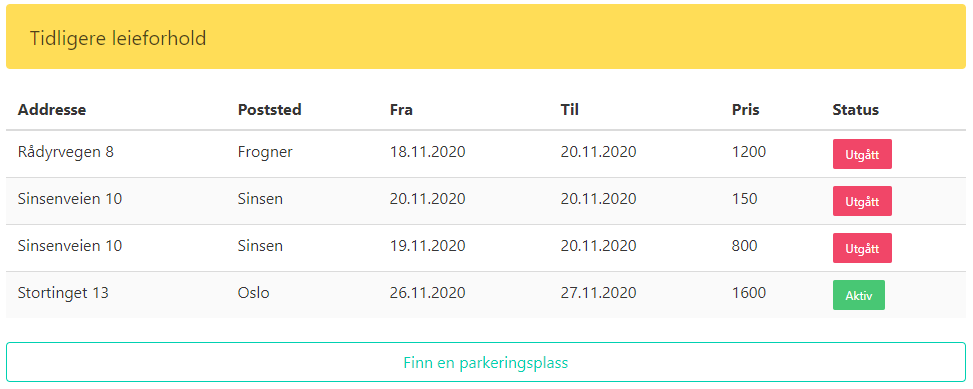
\includegraphics[width=10cm]{bilder/Eksempler/tidligere_leide_plasser.png}
    \caption{Passende tekst}
    \label{fig:eks:profile_leide}
\end{figure}

Det vil bli vist en oversikt over deres tidligere leieforhold. Med en status om parkeringen fortsatt er gyldig eller har utgått.

\begin{figure}[H]
    \centering
    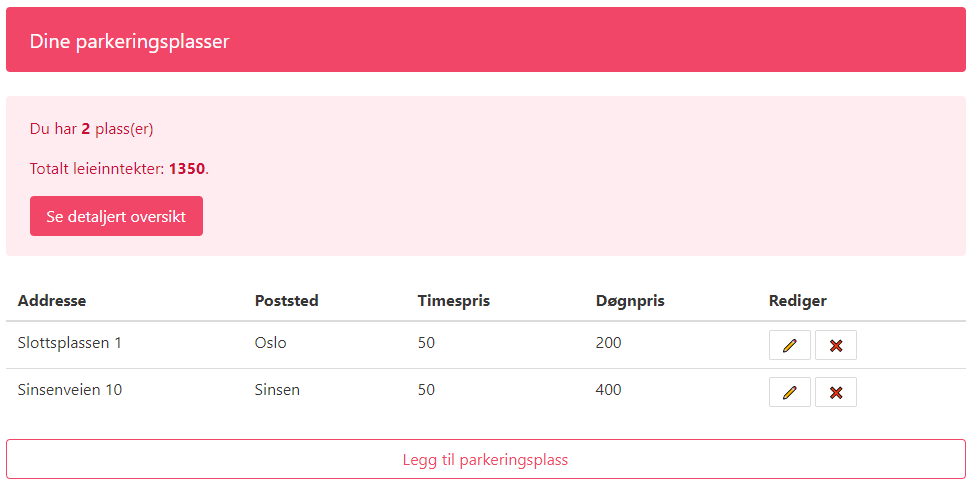
\includegraphics[width=10cm]{bilder/Eksempler/dine_plasser.png}
    \caption{Passende tekst}
    \label{fig:eks:profile_spots}
\end{figure}

Nederst vil de får oversikt over parkeringsplasser de selv leier ut. Og med en samlet inntjening av plassene sine.

\subsubsection{Leie parkeringsplass}
For å leie en plass, trykkes det på knappen «Finn parkeringsplass», som vil ta dem til siden hvor man får en oversikt over tilgjengelige plasser.

\begin{figure}[H]
    \centering
    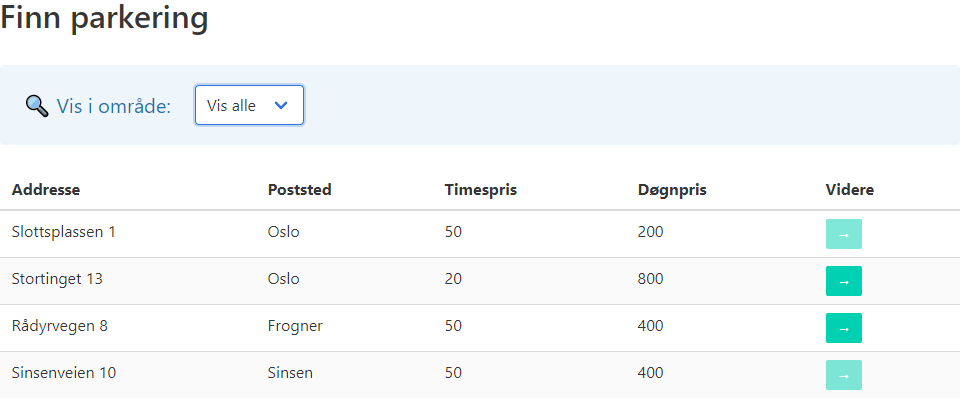
\includegraphics[width=10cm]{bilder/Eksempler/finnparkering.png}
    \caption{Passende tekst}
    \label{fig:eks:findspots}
\end{figure}

Det aktuelle området man leter etter plass kan filtreres ved å bruke nedtrekks menyen. Plasser merket med lysegrønn videre-knapp er brukeren sine egne plasser. Og kan ikke velges.

\begin{figure}[H]
    \centering
    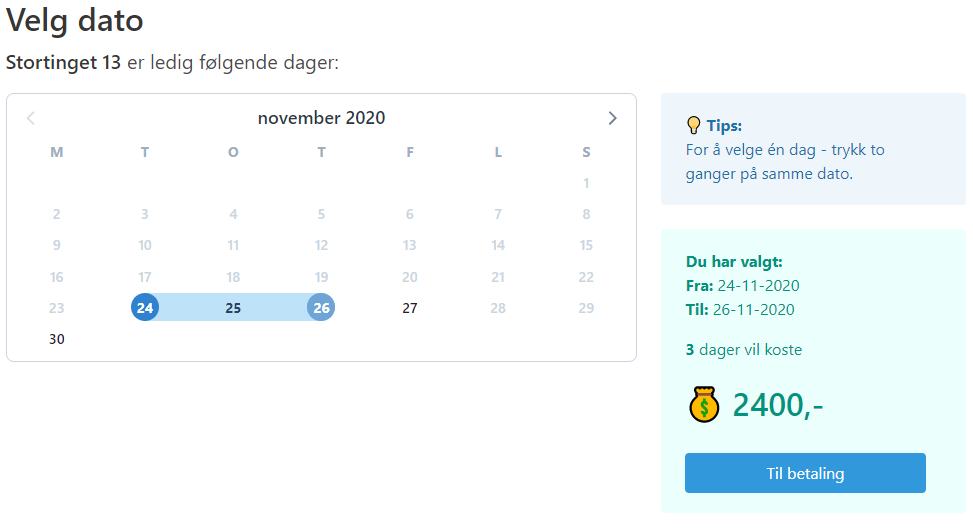
\includegraphics[width=10cm]{bilder/Eksempler/velgdato_dager.png}
    \caption{Passende tekst}
    \label{fig:eks:findspots_days}
\end{figure}

Når brukeren har funnet ønsket plass, velger man tilgjengelig dato i kalenderen. For å leie plass i flere dager velger man til og fra dato. Estimert kostnad for perioden vil bli vist på høyre side.

\begin{figure}[H]
    \centering
    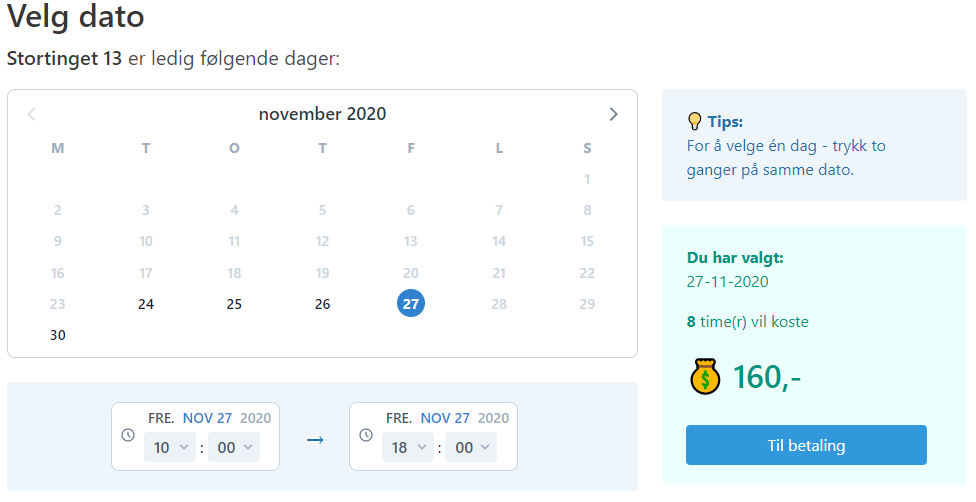
\includegraphics[width=10cm]{bilder/Eksempler/velgdato_timer.png}
    \caption{Passende tekst}
    \label{fig:eks:findspots_hour}
\end{figure}

Hvis det er ønskelig å leie plass kun for noen timer velger man én dato. Det vil da være mulig å spesifisere fra og til klokkeslett de ønsker å leie plassen. Estimert kostnad for perioden vil bli vist på høyre side.

Ved å trykke på «Til betaling» går man videre til betalingssiden.

\begin{figure}[H]
    \centering
    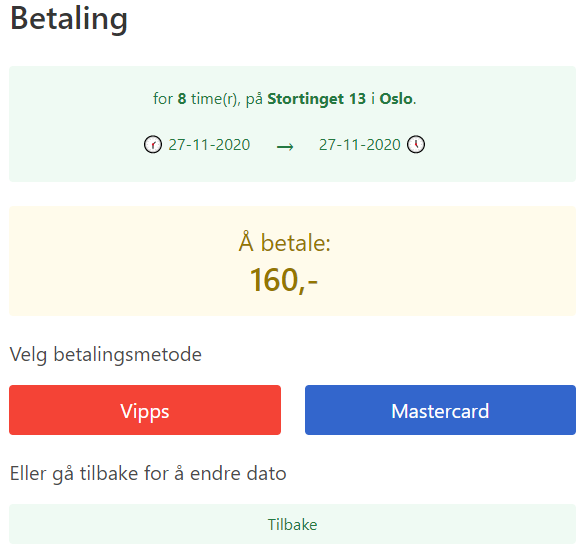
\includegraphics[width=7cm]{bilder/Eksempler/betaling.png}
    \caption{Passende tekst}
    \label{fig:eks:findspots_pay}
\end{figure}

Her blir man vist en oppsummering av bestillingen, og mulighet for å velge betalingsmåte.

\subsection{Installasjon av systemet}
For å installere og bruke systemet kreves Node og en nettleser. Vi har under utvikling brukt \href{https://www.google.com/intl/no/chrome/}{Google Chrome}, og Node versjon v14.13.0. Systemet har også blitt testet og virker med seneste versjon v15.2.1. For å installere Node se fremgangsmåte på deres \href{https://nodejs.org/en/}{hjemmeside}.

Vedlagt produktdokumentasjonen ligger en mappe: «Software-Engineering» som inneholder kildekoden til prototypen. For å fortsette installasjonen av nødvendige avhengigheter trenger vi å åpne terminalen og naviger inn i mappen.

\begin{minted}
[
frame=single,
framesep=10pt,
fontsize=\scriptsize,
breaklines
]
{bash}
$ cd Software-Engineering
\end{minted}

\subsubsection{Server}
Systemet er delt opp i to deler, en \textit{client} og en \textit{server}. Vi skal nå gå igjennom installasjonen av serveren.

I terminalen, naviger inn i \textit{server} mappen, og installer avhengigheter:

\begin{minted}
[
frame=single,
framesep=10pt,
fontsize=\scriptsize,
breaklines
]
{bash}
$ cd server
$ npm install
\end{minted}

\texttt{npm} vill nå laste ned alle avhengigheter til server programmet, og legge disse i mappen \textit{node\_modules}.

Når avhengigheten er ferdig lastet ned er server siden av systemet klart til bruk.

\subsubsection{Client}
Naviger terminalen inn i \textit{client} mappen og installer avhengigheter:

\begin{minted}
[
frame=single,
framesep=10pt,
fontsize=\scriptsize,
breaklines
]
{bash}
$ cd ..\client\
$ npm install
\end{minted}

\texttt{npm} vill nå laste ned alle avhengigheter til klient programmet, og legge disse i mappen \textit{node\_modules}.

Når avhengigheten er ferdig lastet ned er klient siden av systemet klart til bruk.

\subsection{Bruk}
Når avhengigheter til server og klienten er lastet ned og installert er systemet kart til bruk.
\textbf{Merk:} Både \textit{server} og \textit{client} må kjøre for at systemet skal virke som det skal!

\subsubsection{Server}
Vi åpner en ny terminal og navigerer først til \textit{server} mappen. Og starter serveren ved å bruke kommandoen:

\begin{minted}
[
frame=single,
framesep=10pt,
fontsize=\scriptsize,
breaklines
]
{bash}
$ npm run start
\end{minted}

Du vil nå få en tilbakemelding i terminalen som ser slik ut, systemet er klart til bruk på \href{http://localhost:5000}{http://localhost:5000}. Ikke lukk dette terminalvinduet for da avsluttes programmet.

\begin{minted}
[
frame=single,
framesep=10pt,
fontsize=\scriptsize,
breaklines
]
{bash}
> share-a-spot@1.0.0 start
> node index.js

Server running on port: http://localhost:5000
\end{minted}

\textbf{MERK!} Pass på at det ikke er noe annet på maskinen din som allerede kjører på denne porten, dette vill medføre at systemet ikke starter!

Hvis du åpner \href{http://localhost:5000}{http://localhost:5000} i nettleseren din, så skal du se meldingen:
\begin{minted}
[
frame=single,
framesep=10pt,
fontsize=\scriptsize,
breaklines
]
{bash}
{
  message: "Share-A-Spot Server - Up and running"
}
\end{minted}

\subsubsection{Client}
For å starte brukergrensesnittet, åpner vi ett nytt terminalvindu og navigerer til \textit{client} mappen. Vi starter vue sitt utviklingsmiljø ved:
\begin{minted}
[
frame=single,
framesep=10pt,
fontsize=\scriptsize,
breaklines
]
{bash}
$ npm run serve
\end{minted}

Dette vil bygge systemet og gjøre det klart til bruk.
\begin{minted}
[
frame=single,
framesep=10pt,
fontsize=\scriptsize,
breaklines
]
{bash}
App running at:
- Local:   http://localhost:8080/
- Network: http://192.168.1.XXX:8080/

Note that the development build is not optimized.
To create a production build, run npm run build.
\end{minted}

Når det er ferdig vil vi få en tilbakemleding i terminalen at systemet er tilgjengelig på \href{http://localhost:8080}{http://localhost:8080}. Ikke lukk dette terminalvinduet for da avsluttes programmet.

Når begge tjenestene kjører, er systemet klart til å brukes. Du kan nå åpne nettleseren din og navigere til \href{http://localhost:8080}{http://localhost:8080} hvor brukergrensesnittet er.

\subsection{Testing}
Systemet består av et brukergrensesnitt og en API som håndterer forretningslogikk. Det er mot APIen vi har fokusert på å skrive testene. Dette i all hovedsak for at brukergrensesnittet kun viser data som er sendt fra APIen, og det er skal være minimalt med logikk som ligger her.

Vi har skrevet tester mot alle funksjonene i APIen, men ut ifra kildekode oversikten, så er det ett par spesielle punkter hvor vi ikke har gjenskapt enkelte feil-tilfeller. Dette gjelder spesielle tilfeller i noen av funksjonene våre, hvor vi sender en feilmelding tilbake hvis databasen ikke klarer å skrive. Dette scenarioet har vi ikke skrevet en test for. Men logikken for å håndtere det er der. 

En annen test som ikke er fullstendig, er betalingen. Her er det skrevet kode som gjør at betalingen feiler cirka 20\% av gangene. Vi fant ingen løsning for å teste denne funksjonen på en god måte, så det vi gjorde er i stedet var å forvente at systemet ikke feiler, altså ikke gi «500 Internal Server Error». 

\subsubsection{Oversikt over filer}
Testene som tilhører funksjoner forbundet med innlogging finnes i filen \\ \texttt{login.test.js}.

\begin{table}[H]
\centering
\begin{tabularx}{\textwidth}{r|X}
% \begin{tabular}{@{}ll@{}}
4.1.2.a & Logge inn m/ epost-adresse              \\ 
4.1.2.d & Feilmelding ved feil brukernavn/passord \\ 
% \end{tabular}
\end{tabularx}
\end{table}



Brukere skal kunne opprette en konto i tjenesten, og ha en form for brukerprofil med noe funksjonalitet. Tester til følgende krav og funksjoner finnes i filen \texttt{user.test.js}

\begin{table}[H]
\centering
\begin{tabularx}{\textwidth}{r|X}
% \begin{tabular}{@{}ll@{}}
4.1.1.a & Opprette   bruker m/ epost-adresse \\
\ref{bruker_profil}  & Brukerprofil                       \\
% \end{tabular}
\end{tabularx}
\end{table}

Tester til funksjoner relatert til krav om å legge inn og leie plass finnes i filen \texttt{spots.test.js}



\begin{table}[H]
\centering
\begin{tabularx}{\textwidth}{r|X}
% \begin{tabular}{@{}ll@{}}
\ref{Legge_parkering} & Legge inn   parkeringsplass \\ 
\ref{leie_park} & Leie   parkeringsplass      \\
\ref{søke_park} & Søk av   parkeringsplass    \\
\ref{betaling} & Betaling                    \\ 
% \end{tabular}
\end{tabularx}
\end{table}

\subsubsection{Kjøre tester}
For å kjøre testene åpner vi en terminal og navigerer til \texttt{server} mappen. Vi bruker \href{https://jestjs.io/}{Jest} som er ett test rammeverk for JavaScript. Den vil gå igjennom alle mappene å lete etter filer merket med \texttt{<filnavn>.test.js}. Alle filer som ligger i mappen \texttt{\_\_tests\_\_} vil automatisk også bli kjørt. Alle testene til programmet vårt ligger i denne mappen.

Når vi er i \texttt{server} mappen starter vi testene ved:
\begin{minted}
[
frame=single,
framesep=10pt,
fontsize=\scriptsize,
breaklines
]
{bash}
$ npm run test
\end{minted}

Dette vil kun gi oss en tilbakemelding at alle testene var vellykket, eller hvis noen har feilet så vil den gi en tilbakemelding om det. For en mer utdypende rapport bruker vi \texttt{--verbose}. Merk, vi trenger \texttt{--} før \texttt{--verbose}.

\begin{minted}
[
frame=single,
framesep=10pt,
fontsize=\scriptsize,
breaklines
]
{bash}
$ npm run test -- --verbose
\end{minted}

Her får vi nå en oversikt over alle testene som blir kjørt med navnende deres. Disse navnene er også beskrivende slik at det er tydelig hva de tester. Se utdrag fra eksempel:

\begin{minted}
[
frame=single,
framesep=10pt,
fontsize=\scriptsize,
breaklines
]
{bash}
 PASS  __tests__/login.test.js
  GET / *
    OK / - Should respond with 403 - Forbidden (56 ms)
    OK / * (any) - Should respond with 403 - Forbidden (6 ms)
  POST /login
    OK Valid username and password should respond 200 (28 ms)
    OK Invalid username and password should respond 400 (6 ms)
\end{minted}

For få se hvor mye av koden testene faktisk dekker kan vi bruke en annen kommando \texttt{--coverage}.

\begin{minted}
[
frame=single,
framesep=10pt,
fontsize=\scriptsize,
breaklines
]
{bash}
$ npm run test -- --coverage
\end{minted}

Dette vil skape en oversiktlig rapport over hvilke filer som blir testet, hvor mye av koden i filene som blir dekket. Og hvis det er noen deler av koden vi ikke har inkludert. I tillegg lager jest en flott rapport som kan åpnes i nettleseren. Her kan man gå inn i de forskjellige filene, og detaljert se koden, og hvor testene eventuelt ikke dekker. Denne rapporten finner man under \texttt{coverage/Icov-report/index.html}.